\setchapterstyle{kao}
\chapter{Anatomical Contrastive Learning}
\labch{anatcl}

This chapter will discuss the proposed method that is the subject of this
thesis. To set the stage for the discussion, common approaches in deep learning
applied to neuroimaging and related state-of-the-art works will be reviewed.
Following this, the discussion will shift to an explanation of the various steps
and attempts made to extend existing SOTA approaches, ultimately leading to the
final formulation. Furthermore, the results of the conducted experiments will be
discussed.

\section{Related Works}
Until now, the discussion has primarily focused on the supervised framework of
machine learning. In this framework, as previously explained, the model learns
by using a discriminator (a class label) applied to the data. This approach is
particularly effective when large labeled datasets are available. Deep
convolutional models, for instance, require a substantial amount of data to
learn salient features and regularities within the data, especially pertinent to
brain disorders, which involve clinical, biological, and environmental factors.

However, the availability of large-scale labeled datasets poses a significant
challenge, particularly in the medical field~\sidecite{lan_generative_2020}.
Neuroimaging datasets, for example, typically range from a few hundred to a few
thousand participants, which is considerably smaller compared to the datasets
used for training state-of-the-art classification models\sidenote{For instance,
ImageNet~\cite{deng_imagenet_2009} contains more than 14 million images.}. This
limitation becomes even more pronounced for neuroimaging datasets pertaining to
specific rare disorders.

\subsection{Transfer Learning}
Transfer learning has demonstrated to be a powerful tool to overcome these
limitations in the neuroimaging domain, outperforming standard machine learning
approaches in major tasks related to clinical
psychiatry~\sidecite{dufumier_psychiatry_2024}. Instead of directly learning
from a small labeled dataset in a supervised manner, the transfer learning
paradigm employs a two-phased approach. In the first phase, the model
$f_{\theta}$ is trained on a substantial set of image data of healthy
controls\sidenote{Healthy controls are individuals who do not have the condition
or disease being studied and are used as a standard or baseline for comparison
against those who do have the condition, to identify differences related to the
disease.}. During this phase, the CNN model is trained to learn a
low-dimensional embedding space discovering the general variability associated
with non-specific variables such as, for example, age and sex. The feature
extractor can learn to identify various brain features from the image data
present in the dataset. The result of this process is the set of pre-trained
weights $\theta_{HC}$ of the model on the healthy control data. In the
literature of neuroimaging, the pre-training phase has been implemented in
several ways:
\begin{itemize}
    \item \textbf{Contrastive Learning}: this method involves minimizing the
    distance between encoded representations\sidenote{Encoded representations
    are the output of the encoder.} of same-class pairs while maximizing the
    distance between representations of different-class pairs. Classes are
    determined based on the sample label.
    \item \textbf{Autoregressive Learning}: a Variational AutoEncoder (VAE)
    (\reffig{4_1}) is trained to regenerate the same input image.
    Subsequently, the encoder's weights from the learned VAE are utilized as the
    feature extractor's weights in the pre-trained model.
    \item \textbf{Brain Age Prediction}: when data associated with the age of
    the patient is available, the model is trained to predict the real age
    associated with the patient's brain image data (\reffig{4_2}).
\end{itemize}
\begin{figure*}
    \begin{subfigure}[t]{.45\linewidth}
        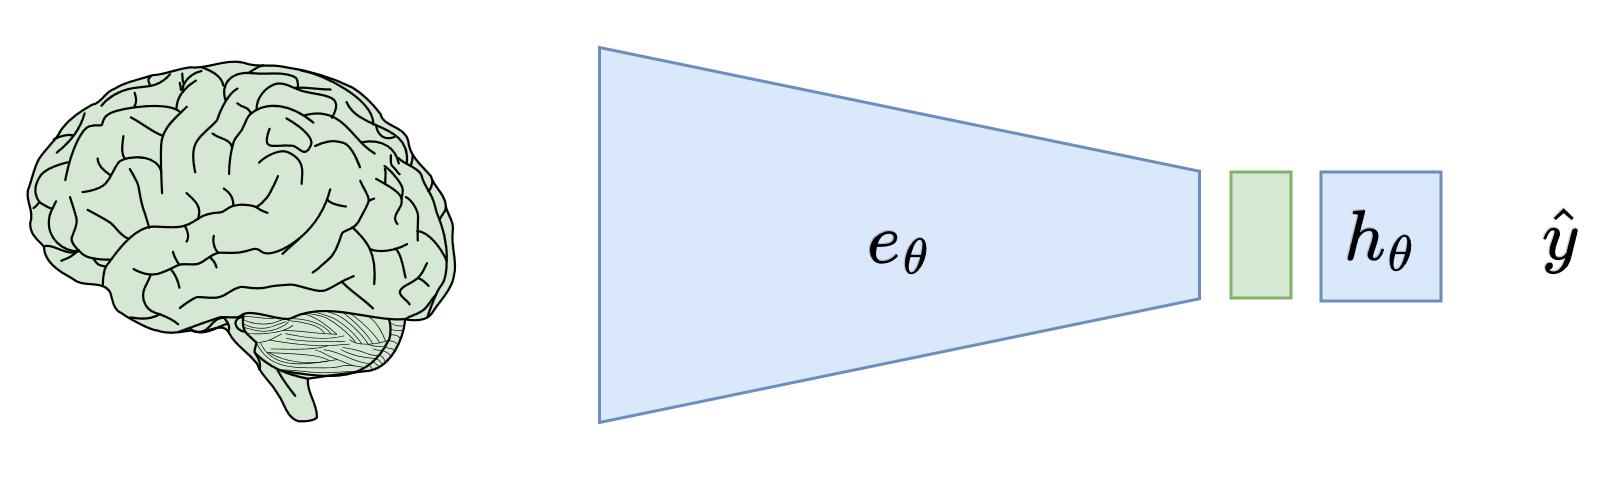
\includegraphics{4_1_age_prediction}
        \caption[Brain Age Prediction Pretraining]{In the brain age prediction
        settings, the encoder $e_\theta$ learns a latent representation of the
        image data that is then used by a discriminator $h_\theta$ to predict
        the age. The predicted age $\hat{y}$ is then confronted with the real
        age $y$ in an appropriate loss function.}
        \labfig{4_1}
    \end{subfigure}
    \hfill
    \begin{subfigure}[t]{.45\linewidth}
        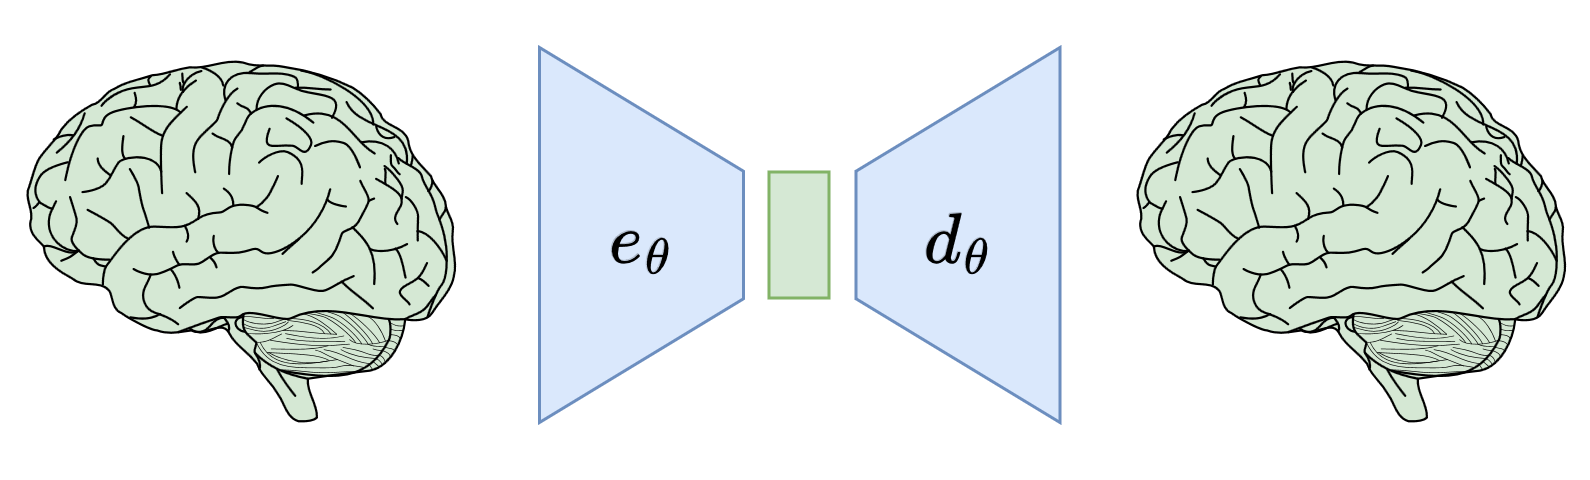
\includegraphics{4_2_vae}
        \caption[Variational Autoencoder Pretraining]{Variational Autoencoders
        consist of an encoder $e_\theta$ that compresses input data into a
        latent space representation (green block) and a decoder $d_\theta$ that
        reconstructs the input data from these encoded representations. In other
        words, the decoder learns to map the latent space back to the original
        data distribution.}
        \labfig{4_2}
    \end{subfigure}
\end{figure*}
After employing the chosen method to pre-train the model, the next phase
involves transferring the trained model on a specific downstream task, using a
dataset of a smaller cohort of patients. Rather than initializing the model
$f_\theta$ with random weights $\theta_{rand}$, it is initialized with the
pre-trained weights $\theta_{HC}$ obtained during the first phase. The
fundamental rationale behind this approach is that by allowing the model to
first learn the general variabilities present in the data, it will requires
significantly less data to subsequently learn the specific features necessary to
distinguish between particular conditions. Although all these pre-training
methods have proven to be extremely effective, a detailed explanation of them is
beyond the scope of this thesis. Given that the current work concentrates on the
contrastive learning framework, it is therefore appropriate to shift the
discussion on this method.

\subsection{Supervised Contrastive Learning}
% TODO: Add another image with augmentation here
\begin{figure}
    \centering
    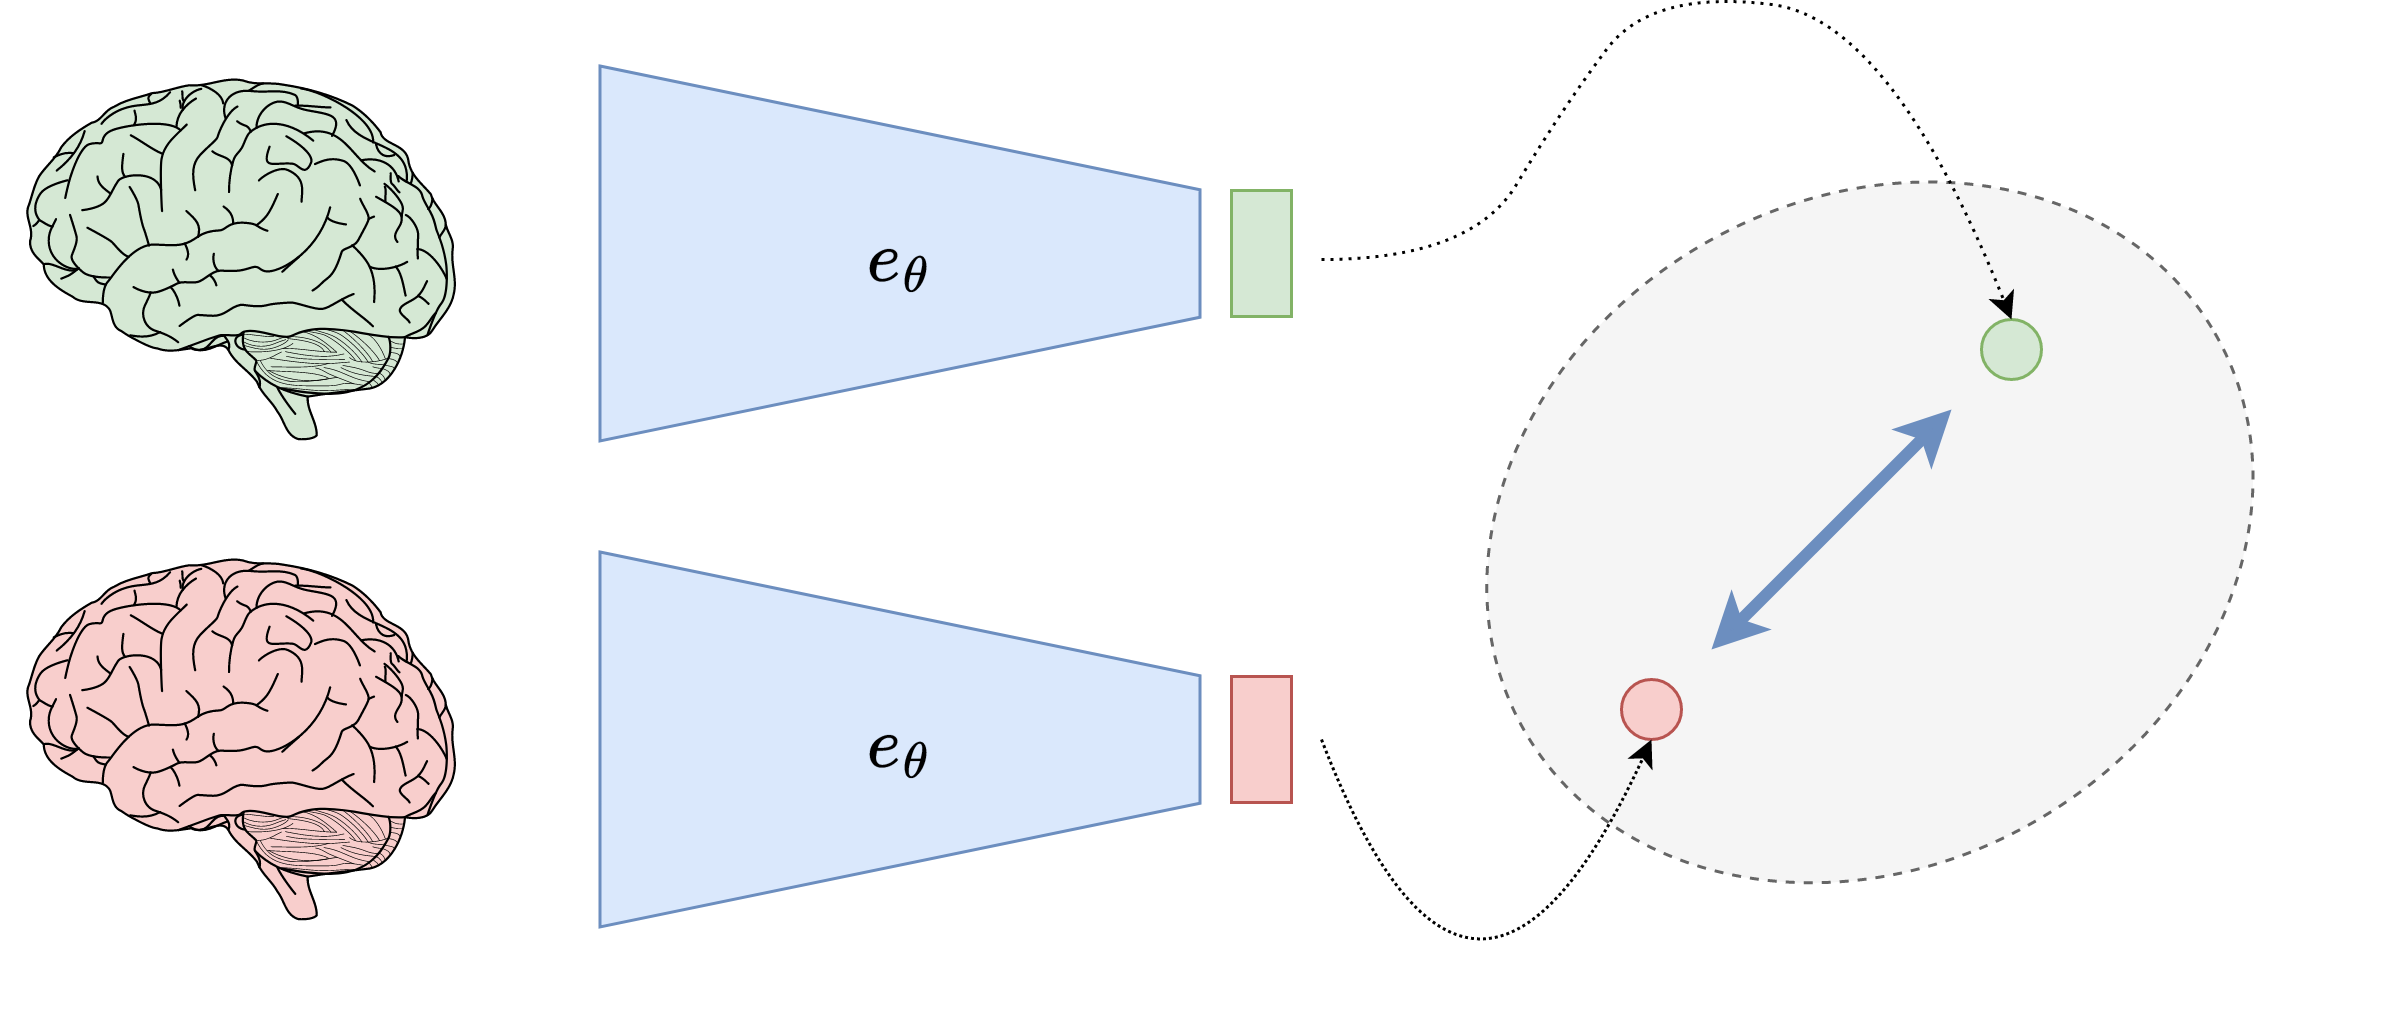
\includegraphics{4_3_contrastive_learning}
    \caption[Contrastive Learning]{The Contrastive Learning method aims at
    maximizing the distance between the latent representations of the anchor
    (green) and the latent representations of negative examples (red).}
    \labfig{4_3}
\end{figure}
As previously mentioned, the foundational principle of the Contrastive
Learning~\cite{hadsell_dimred_2005, chen_self_contrastive_2020,
khosla_supervised_contrastive_2021, henaff_contrastive_2020,
hjelm_contrastive_2019, wu_unsupervised_2018} framework is to develop
representations that draw similar items (positive pairs) nearer in the embedding
space, while distancing dissimilar items (negative pairs). The model
accomplishes this by optimizing a loss function that fosters this specific
behavior. Various loss functions~\cite{schroff_facenet_2015, sohn_improved_2016} have been devised
to foster such behavior, but this discussion will specifically focus on those
used in the supervised context~\sidecite{chen_self_contrastive_2020}. To
establish a more formal foundation for this discussion, consider a neural
network model denoted by $f_\theta$. For any given image and its associated
class label $(x_i, y_i)$ from the dataset, one can compute the latent
representation\sidenote{Also referred to as the \emph{anchor} in this context.}
$z_i = f_\theta(x_i)$. Let also be $I = \{0, \dots, r\}$ the set of indices in
the minibatch, $A(i) = I / i$ the set of indices of all other samples in the
minibatch (except the anchor), and $P(i) = \{p \in A(i) \; : \; y_p = y_i \}$
the set of indices of positive samples\sidenote{Positive in the sense that they
share the same class as the anchor.}.

In the supervised contrastive learning process, each element of the minibatch
$x_i \in \mathcal{B}_r$ is iteratively considered as the anchor. At each step,
each positive sample $x_p$ with $p \in P(i)$ is paired with the anchor to form a
positive pair. Concurrently, the anchor $x_i$ is paired with each remaining
sample $x_a$ with $a \in A(i)$ of the minibatch to form negative pairs. The
objective of the loss is to maximize the similarity\sidenote{Maximizing the
similarity is equivalent to minimizing the distance.} $s_p = sim(z_i, z_p)$
between embeddings of positive pairs, while minimizing the similarity $s_a =
sim(z_i, z_a)$ between negative pairs. The similarity is usually computed though
a \emph{Cosine Similarity}, but can be computed with any similarity measure.
For any anchor $i$, this training objective can be computed using the Supervised
Contrastive (\emph{SupCon}) Loss function, shown in~\refeq{4_1}.
\begin{equation}
    \labeq{4_1}
    \mathscr{L}^{\text{sup}} = 
    - \frac{1}{\lvert P(i) \rvert} \sum_{p \in P(i)} \log \left(
        \frac
        {\exp(s_p / \tau)}
        {\sum\limits_{a \in A(i)} \exp(s_a / \tau)}
    \right)
\end{equation}
Where the term $\tau \in \mathbb{R}^+$ is a scalar value that indicates the
\emph{temperature}\sidenote{The temperature is an hyper-parameter of the loss
function that allows to tune the sensitivity of the loss function to differences
between the distances of positive and negative pairs in the embedding space.} of
the method. The loss of the entire minibatch is simply the sum of the loss
values, considering each element of the minibatch as the anchor.

Models pre-trained with the SupCon loss has shown state of the art accuracy in
classification tasks performed on common labelled imaging
datasets~\cite{chen_self_contrastive_2020}. One of its obvious limitation is
that it needs a large labelled dataset to be applied successfully, which, as
discussed previously, is not the common case of neuroimaging datasets.

\subsection{Self-Supervised Contrastive Learning}
In reality, the SupCon loss is a specific case of a more general function
designed to work in an unsupervised setting. Instead of relying on labels to the
determine the real class of a sample, this method assumes that each sample
belongs to its own unique class. By following this principle, the method applies
an augmentation\sidenote{A series of transformations including cropping,
rotation, and color adjustments, intended to generate a different positive
sample that semantically similar to the original sample but vary in some
features} $Aug(\cdot)$ to the anchor, obtaining another sample $x_j = Aug(x_i)$
that is treated as positive.

The next step is equivalent to the SupCon loss. A positive pair is formed by
means of augmentation to the anchor, and negative pairs are formed using all the
remaining samples in the minibatch. \refeq{4_2} summarizes the Self Supervised
Contrastive loss function.
\begin{equation}
    \labeq{4_2}
    \mathscr{L}^{\text{self}} = - \log \left(
        \frac
        {\exp(s_j / \tau)}
        {\sum\limits_{a \in A(i)} \exp(s_a / \tau)}
    \right)
\end{equation}
Technically speaking, minimizing these loss formulations corresponds to
maximizing the mutual information~\cite{aaron_representation_2018} between
positive pair representations, effectively increasing the amount of shared
information between a positive representation $(z_i)$ and its augmented sample
$(z_j)$. \refeq{4_2} can also be interpreted from a probabilistic perspective.
Through this lens, the numerator can be seen as assigning a high probability to
the event where the anchor and its positive pair are close together in the
embedding space. The denominator acts as a normalization factor, summing the
exponential similarity scores of the anchor with all other embeddings in the
batch (except for itself). This sum transforms the raw exponential scores into
probabilities via the softmax function, thus creating a probability
distribution\sidenote{Also referred to as the \emph{noise} distribution, as it
should include negative samples.} over all pairs involving the anchor and a
negative sample, where pairs with higher similarity scores are assigned higher
probabilities. In essence, the ratio calculates the probability that the anchor
$z_i$ is similar to the positive embedding $z_j$, relative to the probability of
being similar to any other negative embedding $z_a$.

The role of the numerator is to create a "pulling" force between the anchor and
its positive counterpart in the embedding space, ensuring that these connections
are reinforced more strongly during the training process than any other
connections. Conversely, the denominator serves to "push" negative samples away
from the anchor in the embedding space.

However, viewing these loss functions from a probabilistic angle also highlights
a potential issue. These losses assume that all other samples in the minibatch,
aside from the anchor, are negative samples, even though there may be
semantically similar samples to the anchor present in the minibatch. In other
words, other potentially positive samples could be inadvertently included in the
noise distribution.

\subsection{Weakly-Supervised Contrastive Learning}
To address the issue of false negatives in the noise distribution, several
studies have proposed modifications to the aforementioned loss functions. These
adjustments are classified under the umbrella of weakly supervised strategies.
The essence of these strategies is to utilize additional metadata associated
with a sample to define closeness in the embedding space. The underlying
intuition is that samples from similar classes would also share similar
characteristics and, consequently, similar metadata. Augmenting the loss
functions with additional information helps refine the distinction between
positive and negative pairs, improving the effectiveness of the model in
recognizing and differentiating between closely related samples.

In the neuroimaging domain,
\citeauthor{dufumier_contrastive_2021}~\sidecite{dufumier_contrastive_2021}
proposed a method that incorporates the age of a patient associated with a brain
scan as additional metadata. In their research, a contrastive loss function
named \emph{y-aware}\sidenote{This term is used because the model utilizes the
target variable $y$ during the pre-training phase.} was developed. The
fundamental concept of this function is to calculate a weight term $0 \leq w_k
\leq 1$ that determines the \emph{degree of positiveness} of the $k^{th}$ sample
relative to the anchor. To compute this term, the authors suggest applying a
kernel\sidenote{Which could either be a Gaussian or RBF kernel.} $K_\sigma$ to
the age difference between the patients associated with the brain images.
Formally, if $y_k$ is the age attribute associated with the $k^{th}$ sample,
then the weight term is calculated as shown
in~\refeq{4_3}.
\begin{equation}
    \labeq{4_3}
    w_k = K_\sigma(y_i - y_k)
\end{equation}
The role of the kernel $K_\sigma$ in this context is to constrain the difference
value between 0 and 1. The hyper-parameter $\sigma$ determines the spread of the
kernel and can be readily estimated from the dataset.

The weight term $w_k$ is subsequently incorporated into the SupCon loss
formulation by multiplying each pair by its corresponding weight
value\sidenote{Indeed, the original formulation in \refeq{4_1} is a special
case of the \emph{y-aware} function, where weights are implicitly set to either
$1$ or $0$, depending on whether $x_k$ belongs to the same class as $x_i$ or
not.}. This modification allows the model to adjust the influence of each sample
pair in the loss calculation based on their relative age difference.
\refeq{4_4} shows the formulation of the \emph{y-aware loss}.
\begin{equation}
    \labeq{4_4}
    \mathscr{L}^{\text{y-aware}} = 
    -\sum_{k \in A(i)} \frac{w_k}{\sum_t w_t} log
    \left(
    \frac
    {\exp(s_k / \tau)}
    {\sum\limits_{a \in A(i)} \exp(s_a / \tau)}
    \right)
\end{equation}
Pre-trained models that employ the \emph{y-aware} loss have subsequently
achieved state-of-the-art performance in downstream tasks involving the
prediction of neurological pathologies such as Schizophrenia (SCZ), Bipolar
Disorder (BD), and Alzheimer's Disease (AD).

Subsequent research has further explored refinements of the \emph{y-aware} loss
concept. Specifically,
~\citeauthor{barbano_contrastive_2023}~\sidecite{barbano_contrastive_2023}
proposes two extensions to the original formulation. The first refinement arises
from the observation that the uniformity term (the denominator) in \refeq{4_4}
tends to focus more on the closest samples within the representation space. This
concentration means that if positive samples exist elsewhere in the minibatch,
they are inadvertently included in the noise distribution, thus receiving
disproportionately high weighting compared to other negative samples. To address
this issue, the uniformity term is adjusted to include only those samples that
are more distant from the anchor than the considered $x_k$ in the kernel
space. This refinement helps ensure that the term focuses on truly negative
samples, thereby reducing the influence of inadvertently included positive
samples in the noise distribution. \refeq{4_5} shows the proposed loss
function that encodes this behaviour.
\begin{equation}
    \labeq{4_5}
    \mathscr{L}^{\text{thr}} = 
    -\sum_{k \in A(i)} \frac{w_k}{\sum_t \delta_{w_t < w_k} w_t} \log
    \left(
    \frac
    {\exp(s_k / \tau)}
    {\sum\limits_{a \in A(i)} \delta_{w_t < w_k} \exp(s_a / \tau)}
    \right)
\end{equation}
Where $\delta_{c}$ is a step function whose value are $1$ when the condition
$c$ is true or $0$ otherwise.

The other loss function proposed takes an opposite approach. Rather than
repelling the closest "least positive" sample, it adjusts the repulsion strength
(i.e., the weight) on the noise distribution in proportion to their distance
from the anchor in the kernel space. This method ensures that samples farther
away from the anchor exert a greater influence on the noise distribution,
thereby refining how the model discriminates between truly negative and
potentially positive samples within the embedding.
\begin{equation}
    \labeq{4_6}
    \mathscr{L}^{\text{exp}} = 
    -\sum_{k \in A(i)} \frac{w_k}{\sum_t w_t} \log
    \left(
    \frac
    {\exp(s_k / \tau)}
    {\sum\limits_{a \in A(i)} \exp((1 - w_t) s_a / \tau)}
    \right)
\end{equation}
In~\refeq{4_6}, which encapsulates this concept, the weighting factor $(1 -
w_t)$ serves as a negative weighting factor, assigning more weight to samples
that are farther from the anchor in the kernel space. This adjustment emphasizes
the influence of distant samples in the kernel space, effectively pushing them
away from the anchor in the embedding space.

To evaluate these loss functions, a 3D CNN was trained specifically to minimize
the loss function under consideration. After the training of the CNN, a linear
classifier was then trained on the latent representations produced by the CNN,
using a smaller validation dataset. Essentially, the CNN model functions to map
brain images into a more compact representation space, from which a linear
classifier is subsequently trained. In the experiments conducted, the downstream
task for which the linear classifier was trained is brain-age prediction. This
approach allows to assess the effectiveness of the latent space learned by the
CNN and to determine how well the extracted features contribute to estimating
brain age. The experiments conducted demonstrated that the loss function
$\mathcal{L}^{exp}$ yielded superior results, suggesting that
$\mathcal{L}^{exp}$ effectively facilitates the extraction and encoding of
relevant features, that improves the model's predictive capabilities on the
brain-age prediction task.

All of these weakly supervised loss functions have shown promising experimental
results; however, a notable limitation of this class of approaches is their
reliance on a single attribute, such as age, to determine the alignment strength
($w_k$). Consequently, they are not well-suited to leveraging multiple
attributes, such as anatomical measurements of the brain. The method proposed in
the subsequent section addresses this limitation by extending the weakly
contrastive formulation to include multiple attributes, thereby enhancing the
model’s capacity to capture and utilize a broader spectrum of relevant
information.

\section{AnatCL}
To extend the discussed loss functions to include multiple attributes, one of
the initial approaches undertaken involved directly modifying the weight
computation. A straightforward and quick method to consider is to define the
weight as the average of the kernelized differences between each selected
attribute. More formally, if the target attribute $y$ is not just a single
scalar but a vector $\mathbf{y}$ consisting of $L$ attributes, the resulting
weight $w_k$ could be calculated using~\refeq{4_7}.
\begin{equation}
    \labeq{4_7}
    w_k = \frac{1}{L} \sum_{l=0}^{L} K_l ( \mathbf{y}_{i,l} - \mathbf{y}_{k, l} )
\end{equation}
This formulation applies the kernel $K_l$ to the difference between each
attribute $l$ to derive an attribute-wise similarity value. Subsequently, the
mean of these similarity values is calculated to produce a single scalar value.
The mean operation is done to ensures that each attribute contributes equally to
the overall weight, allowing for a balanced integration of multiple
characteristics. Also, in order to accommodate the unique variabilities
associated with each attribute, a different kernel $K_l$ is applied to each
difference.
This initial formulation was first tested using a set of selected
attributes—namely age, CerebroSpinal Fluid Volume (CSFV), Gray Matter Volume
(GMV), and White Matter Volume (WMV)—made available by the OpenBHB
dataset~\sidecite{dufumier_openbhb_2022}. To evaluate the effectiveness of this
new formulation, a 3D ResNet-18 model was pre-trained using this contrastive
loss formulation on the OpenBHB dataset. Subsequently, the model was tested on
the brain-age prediction task using a test split of the dataset. Although this
first approach incorporates more information into the learning process, it
demonstrated a decline in performance compared to counterparts that utilize only
the single age attribute\sidenote{More precisely, in the downstream task of
brain age prediction, the mean squared error (MSE) recorded was 7.29, in
contrast to a significantly lower MSE of 2.66 achieved with the baseline
method.}. The hypothesis is that these anatomical attributes are global features
of the brain that may act as confounders for the
model~\sidecite{komeyer_framework_2024}.

The suboptimal performances observed with this formulation highlighted the need
for a different approach to address this problem. Attention shifted specifically
to another set of anatomical features derived from
the~\citeauthor{desikan_automated_2006} brain
parcellation~\sidecite{desikan_automated_2006}. As previously discussed
in~\refch{neuroimaging}, the Desikan brain parcellation is represented
by a matrix $\mathcal{D} \in \mathbb{R}^{68 \times 7}$, where each row contains
a vector of $7$ features. Each vector represents a set of anatomical features
measured in a specific brain area. Despite offering a richer and more nuanced
representation of anatomical features, the Desikan parcellation presents
challenges due to the multi-dimensional nature of its data. This complexity
poses difficulties in formulating an effective similarity measure, as the
previously discussed loss formulations have primarily addressed scalar feature
values. To incorporate these measurements effectively, it is essential to define
a robust similarity measure between two Desikan parcellations.

\subsection{Local Descriptor}
Two different formulations were hypothesized based on the interpretation of the
Desikan parcellation. The first arises from viewing the Desikan parcellation as
comprised of $68$ vectors of $7$ anatomical measurements. According to this
interpretation, the proposed method to compare two parcellations involves
calculating the pairwise similarity between each corresponding measurement,
resulting in a vector of $68$ similarity values. Each value in this vector
indicates the degree of closeness between the corresponding brain regions in
terms of the recorded anatomical features. Finally, the expected similarity
value across all measurements is then used as the degree of positiveness that
can be subsequently used in one of the weakly contrastive loss formulations
discussed earlier. Since with this interpretation the degree of positiveness is
obtained by computing the expected value of the cross-region similarities, it
has been called \emph{"local descriptor"}.
\begin{figure*}[t]
    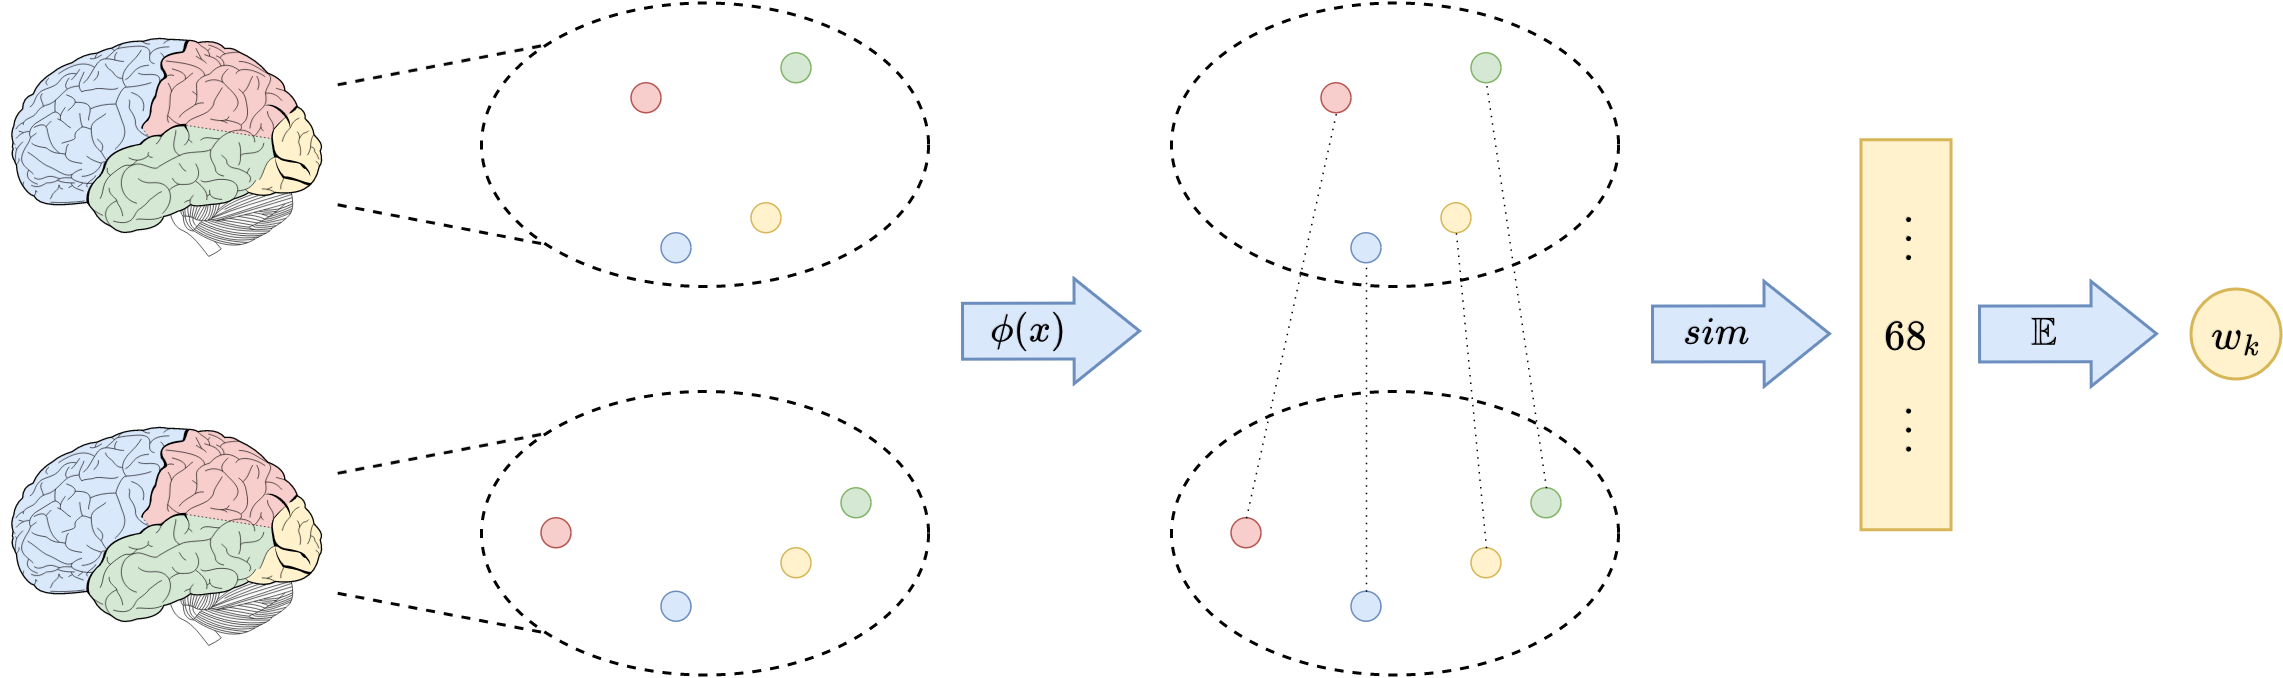
\includegraphics{4_4_local_descriptor}
    \caption[Local Descriptor]{Graphical depiction of the steps required to compute the local
    descriptor. In this interpretation, two different Desikan parcellations are
    visualized as a series of 68 points within a 7-dimensional space. The first
    step in computing the local descriptor involves normalizing these vectors
    through the function $\gamma(x)$, ensuring that they are positioned on the
    unit hypersphere. Following normalization,
    the next step involves calculating the pairwise similarities between each
    measurement vector, resulting in a vector of 68 similarity values. Each
    value reflects the closeness between corresponding brain regions in terms of
    their anatomical features. To determine the final degree of positiveness,
    which quantifies the overall similarity between the two parcellations, the
    expected value $\mathbb{E}$ is computed across the similarity vector.
    }
    \labfig{4_4}
\end{figure*}
Formally, the Desikan parcellation of a $i^{th}$ sample is represented as
$\mathcal{D}^i \in \mathbb{R}^{68 \times 7}$. Each row $\mathcal{D}^i_n$ denotes
the measurement vector for the $n^{th}$ brain region of the $i^{th}$ patient.
Before proceeding with cross-similarity calculations, an adjustment must be made
due to the fact that each feature within a measurement vector captures specific
anatomical information and is recorded on a scale that differs from other
measurements within the vector. To address this variability, a
normalization\sidenote{A transformation used to re-scale values to a range of
$[0;1]$. An example of a normalization is the min-max normalization.}
$\gamma(x)$ is applied to each vector to standardize all measurements.
Following this approach, \refeq{4_8} illustrates the formulation of the
discussed local descriptor.
\begin{equation}
    \labeq{4_8}
    w_k = \frac{1}{68}\sum_{n=1}^{68} sim(\gamma(\mathcal{D}^i_n), \gamma(\mathcal{D}^k_n))
\end{equation}
Where $sim(x, y)$ can be any similarity function\sidenote{In this work the
Cosine Similarity has been mainly used.}. In this case, the $w_k$ term
calculates the atlas-wise similarity of the $k^{th}$ parcellation in relation to
the anchor parcellation $i$.

\subsection{Global Descriptor}
The global descriptor derives from interpreting the Desikan format from another
point of view. Rather than viewing the data as 68 measurement vectors, each
containing 7 different features, this approach considers the format as 7 feature
vectors, each composed of 68 measurement values. Each vector encompasses the
values of a specific measurement recorded across all 68 brain areas. This
reorganization shifts the focus from the regional to the feature-specific
analysis, facilitating a global evaluation that highlights how each individual
anatomical characteristic varies across different brain regions. In other words,
this interpretation arises from considering the transposed version of the
Desikan parcellation, denoted as $\mathcal{D}^T$, which transforms the matrix
into a $7 \times 68$ dimensional format. This transposition shifts the focus from
regional measurements to a feature-centric analysis, allowing each row of the
matrix to represent all the measurements of a specific feature across the 68
brain regions.
\begin{figure}[t]
    \caption[Global Descriptor]{In the corresponding visualization, each brain,
    colored distinctively, represents a specific feature vector, which can be
    depicted in a 68-dimensional space. The global descriptor involves computing
    the cross-similarity, resulting in a 7-element vector that contains
    feature-wise similarities. Similar to the local descriptor, the expected
    value of this vector is calculated to determine the degree of positiveness.}
    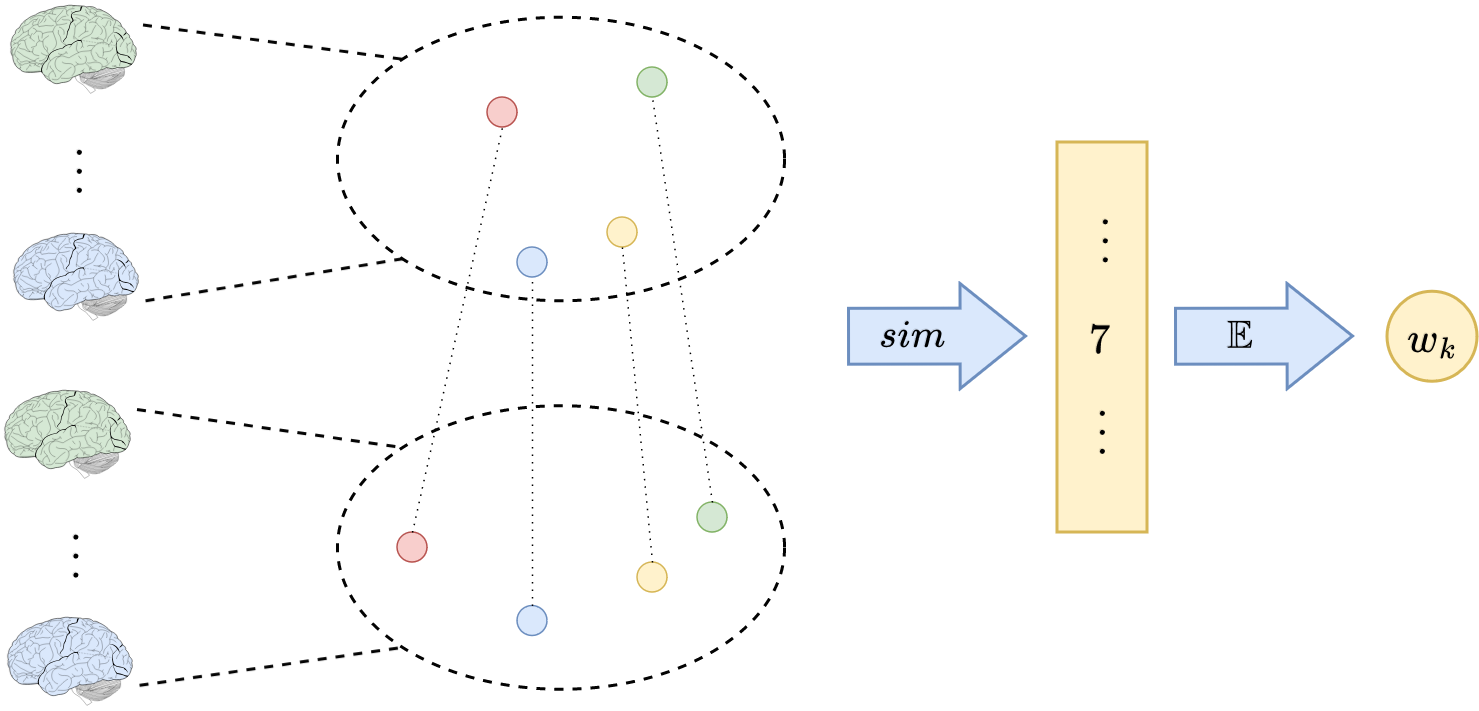
\includegraphics{4_5_global_descriptor}
    \labfig{4_5}
\end{figure}
Since each row of the transposed $\mathcal{D}^T$ matrix contains measurements of
a specific feature across different regions, all data are maintained on a
consistent scale. This uniformity across each vector means that no normalization
step is required before computing the similarity values, simplifying the process
and ensuring that the original measurement scales are preserved during analysis.
\refeq{4_9} shows the formulation of the global descriptor, where $\omega^i_n
= \left( \mathcal{D}^i \right)^T_n$ is the row vector of the transposed
parcellation of the $i^{th}$ sample, containing the 68 measurements pertaining
the $n^{th}$ feature.
\begin{equation}
    \labeq{4_9}
    w_k = \frac{1}{7}\sum_{n=1}^{7} sim(\omega^i_n, \omega^k_n)
\end{equation}
Both the local and global descriptor can then be utilized to calculate the $w_k$
term in one of the weakly supervised contrastive loss formulations previously
discussed. Given that this loss relies on anatomical measures, it has been
designated as $\mathcal{L}^{\text{AnatCL}}$.

To incorporate also the age attribute into the final objective loss, the
resulting function is structured as a weighted sum. This sum combines a weakly
supervised loss that is augmented with the age attribute
($\mathcal{L}^{\text{age}}$) and another weakly supervised loss that utilizes
the anatomical information ($\mathcal{L}^{\text{AnatCL}}$). The specific
formulation of this final objective loss is detailed in \refeq{4_10}.
\begin{equation}
    \labeq{4_10}
    \mathcal{L} = \lambda_1 \mathcal{L}^{\text{age}} + \lambda_2 \mathcal{L}^{\text{AnatCL}}
\end{equation}
In the formulation of the final objective loss function,
$\mathcal{L}^{\text{age}}$ represents any of the previously discussed weakly
supervised loss functions where the computation of the degree of positiveness is
determined using the age attribute. Conversely, $\mathcal{L}^{\text{AnatCL}}$
refers to a weakly supervised loss where the degree of positiveness is computed
using either the local or global descriptor, depending on the specific
anatomical features considered.
Additionally, $\lambda_1, \lambda_2 \in \mathbb{R}$ serve as scalar
hyper-parameters within the loss function. These parameters are used to weigh
the importance of each loss component, thereby determining the preference
between \(\mathcal{L}^{\text{age}}\) and \(\mathcal{L}^{\text{AnatCL}}\).
Adjusting these values allows for fine-tuning of the model's sensitivity to
either the chronological age or the anatomical features, optimizing the balance
based on specific predictive goals or dataset characteristics. 
\begin{figure}
    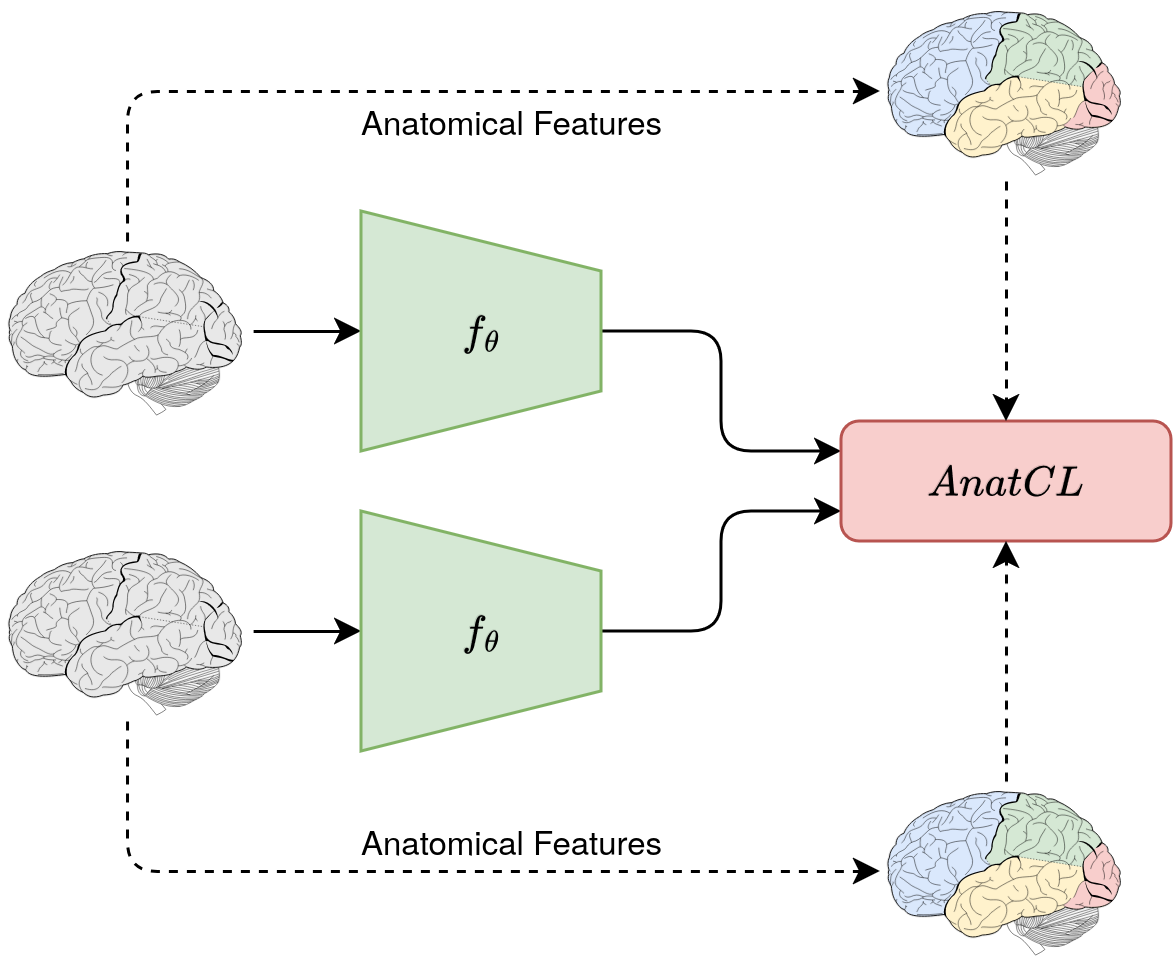
\includegraphics[width=.7\linewidth]{4_6_anatcl_framework}
    \caption[AnatCL Loss Overview]{AnatCL loss overview.}
    \labfig{4_6}
\end{figure}